\section{Experiments}\label{s:experiments}
All experiments have been conducted on a CPU with Intel(R) Core(TM) i5-7200U (@ 2.50 GHz) having 8 GB RAM and running Windows 10 operating system. For applying various ranker algorithms, Weka 3.9 \cite{weka} has been used. We evaluate the performance of the models using F-score. F-score is a popular and reliable metric that is widely used in the literature. In fact we report the weighted average F-score in the range of [0,1] ($F_{wa}$) which is defined as follows:

\begin{equation}
F_{WA} = \frac{F_{Alive} * Count_{Alive} +  F_{Dead} * Count_{Dead}}{Count_{Alive} + Count_{Dead}}
\end{equation} 

\subsection{Feature sets for MIMIC-II and MIMIC-III}
\textcolor{blue}{For MIMIC-II datasets, 655 lab tests are identified and these are treated as feature sets for the experiments on MIMIC-II datasets. On the other hand, 570 lab tests are collected and these are used for the experiments on MIMIC-III datasets. The detail list of these lab tests are available int the supplementary file.}
 
\subsection{Notations/Definitions used to represent the results}
The notations defined in Table \ref{t:resultnotations0} and Table \ref{t:resultnotations} are used to present the results.

\begin{table}[h] 
	\centering \caption{Description of some notations used in results} 
	\begin{tabular}{|p{1.25cm}|p{6cm}|p{0.2cm}|p{1.25cm}|p{6cm}|}\hline
		\textbf{Notation} & \textbf{Description} & & \textbf{Notation}  & \textbf{Description} \\\hline
		J48 & J48 classifier & & FVC & Feature Vector Compaction\\\hline
		NB & NaiveBayes classifier & & H & Horizontal clustering \\\hline
		RF & RandomForest classifier & & V & Vertical clustering \\\hline
		SVM & Support vector machine classifier & & HV & First Horizontal and then Vertical clustering \\\hline
		VC & Vacuum Count method & & VH & First Vertical and then Horizontal Clustering \\\hline
		CFC & Common Feature Count method & & & \\\hline  	
	\end{tabular}
	\label{t:resultnotations0}
\end{table}

\begin{table}[h] 
	\centering \caption{Description of ranking notations used in results} 
	\begin{tabular}{|c|c|}\hline
		\textbf{Notation}  & \textbf{Description} \\\hline
		NoR & No Ranking method applied \\\hline
		R1 & $1^{st}$ subset of features by InfoGain ranker. Zero merit valued features are removed. \\\hline
		R1-1 & $2^{nd}$ subset of features by InfoGain ranker. $1/4$ of total ranked features are kept for experiment. \\\hline
		R1-2 & $3^{rd}$ subset of features by InfoGain ranker. $1/2$ of total ranked features are kept for experiment. \\\hline
		R1-3 & $4^{th}$ subset of features by InfoGain ranker. $3/4$ of total ranked features are kept for experiment. \\\hline
		R2 & $1^{st}$ subset of features by Correlation ranker. Zero merit valued features are removed. \\\hline
		R2-1 & $2^{nd}$ subset of features by Correlation ranker. $1/4$ of total ranked features are kept for experiment. \\\hline
		R2-2 & $3^{rd}$ subset of features by Correlation ranker. $1/2$ of total ranked features are kept for experiment. \\\hline
		R2-3 & $4^{th}$ subset of features by InfoGain ranker. $3/4$ of total ranked features are kept for experiment. \\\hline
		R3 & $1^{st}$ subset of features by RandomForest ranker. Zero merit valued features are removed. \\\hline
		R3-1 & $2^{nd}$ subset of features by RandomForest ranker. $1/4$ of total ranked features are kept for experiment. \\\hline
		R3-2 & $3^{rd}$ subset of features by RandomForest ranker. $1/2$ of total ranked features are kept for experiment. \\\hline
		R3-3 & $4^{th}$ subset of features by RandomForest ranker. $3/4$ of total ranked features are kept for experiment. \\\hline
		R4 & $1^{st}$ subset of features by SVM ranker. Zero merit valued features are removed. \\\hline
		R4-1 & $2^{nd}$ subset of features by SVM ranker. $1/4$ of total ranked features are kept for experiment. \\\hline
		R4-2 & $3^{rd}$ subset of features by SVM ranker. $1/2$ of total ranked features are kept for experiment. \\\hline
		R4-3 & $4^{th}$ subset of features by InfoGain ranker. $3/4$ of total ranked features are kept for experiment. \\\hline
	\end{tabular}
	\label{t:resultnotations}
\end{table}

\subsection{Experiments with variations}
For each dataset, multiple ensemble models are created. In particular, for each dataset, 4 separate subsets of high ranked features, produced by 4 different feature ranking algorithms, are combined with four combinations of feature vector grouping, namely, HV (i.e., ORCU-HV), H (i.e., Horizontal), VH (i.e., ORCU-VH), V (i.e., Vertical). Thus a number of models with different combinations are constructed. We refer to these models using the following form: Model$_{<i>}^{<datasetID-combination>}, 1\leq i \leq 572$. Figure \ref{F:ModelGenOverview} shows how these 572 models are generated for each dataset. For example, Model$_\mathrm{i}^\mathrm{AF-R1HVCJ48}$ refers to the model where (a) Adult Binary (F) dataset is used for training \& testing; (b) $1_{st}$ subset of the ranked features (i.e., R1) are used after applying a ranking algorithm; (c) \textit{Horizontal} feature vector compaction has been applied; (d) Vacuum count has been used and (e) J48 has been employed as the classifier algorithm.

\begin{figure}[h] 
	\centering 
	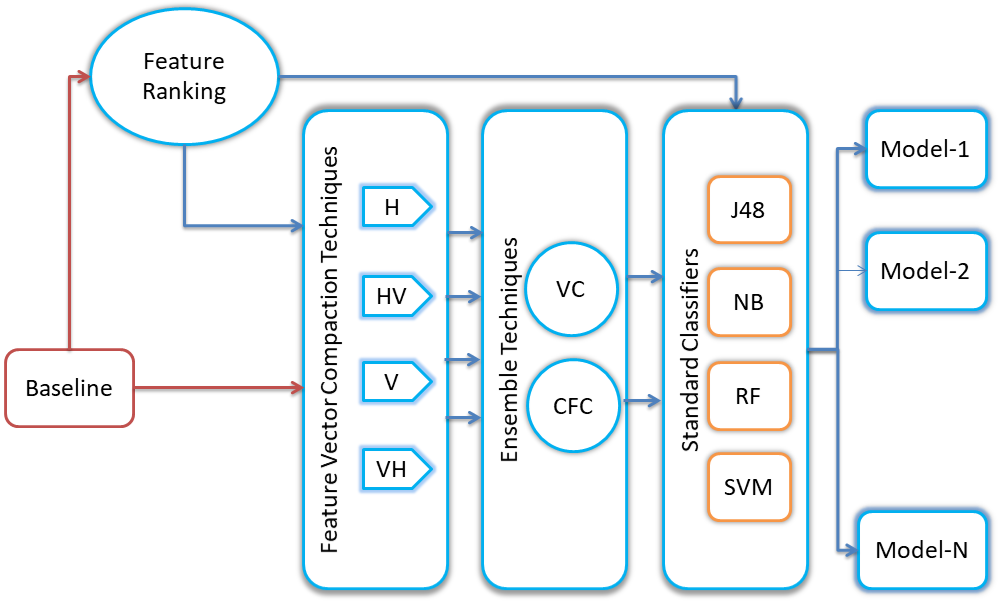
\includegraphics[scale=0.5]{fig/ModelGenOverview.png}
	\caption{Model Generation Overview}
	\label{F:ModelGenOverview}
\end{figure}

So, all considered approaches are listed in Table \ref{t:competingmodels}. Additionally, we have constructed the baseline model using all the features, i.e., ignoring the feature ranking exercise; this model is referred to as Model$_{Base}^{<datasetID>}$.

\begin{table}[h] 
	\centering \caption{Competing approaches} 
	\begin{tabular}{|c|c|c|c|}\hline
		\textbf{Name/Acronym} & \textbf{Reference} & \textbf{Data grouping} & \textbf{Ensambling} \\\hline
		Baseline 1/BL1 & - & - & - \\\hline
		Baseline 2/BL2 & \cite{mehedy-masud:2017:fvc} & FVC & VC \\\hline
		Baseline 3/BL3 & \cite{mehedy-masud:2018:frmwrk} & ORCU-VH & VC \\\hline
		Model$_{<i>}^{<datasetID-combination>}, 1\leq i \leq 3144$ & This study & Horizontal, Vertical, ORCU-VH, ORCU-HV & VC,CFC \\\hline 
	\end{tabular}
	\label{t:competingmodels}
\end{table}
